%% 
%% Copyright 2019-2021 Elsevier Ltd
%% 
%% This file is part of the 'CAS Bundle'.
%% --------------------------------------
%% 
%% It may be distributed under the conditions of the LaTeX Project Public
%% License, either version 1.2 of this license or (at your option) any
%% later version.  The latest version of this license is in
%%    http://www.latex-project.org/lppl.txt
%% and version 1.2 or later is part of all distributions of LaTeX
%% version 1999/12/01 or later.
%% 
%% The list of all files belonging to the 'CAS Bundle' is
%% given in the file `manifest.txt'.
%% 
%% Template article for cas-sc documentclass for 
%% single column output.

\documentclass[a4paper,fleqn,review]{cas-sc}

% If the frontmatter runs over more than one page
% use the longmktitle option.

%\documentclass[a4paper,fleqn,longmktitle]{cas-sc}

\usepackage[numbers]{natbib}
%\usepackage[authoryear]{natbib}
%\usepackage[authoryear,longnamesfirst]{natbib}

%my packages 
\usepackage{lineno,hyperref}

\usepackage{mhchem}
\usepackage{gensymb}
\usepackage{graphicx}

\graphicspath{{figures/}}


\usepackage{epstopdf}
\usepackage{subfig}
\usepackage{xcolor}
\usepackage{siunitx}
\usepackage{nicefrac}

\usepackage{tikz}
\newcommand{\redcircle}{\tikz\fill[red] (0,0) circle (1.5pt);}

\tikzset{
	dotdash/.style={dash pattern=on 3pt off 2pt on 0.5pt off 2pt}
}

\usepackage{threeparttable}
\usepackage{caption}

%%%Author macros
\def\tsc#1{\csdef{#1}{\textsc{\lowercase{#1}}\xspace}}
\tsc{WGM}
\tsc{QE}
%%%

% Uncomment and use as if needed
%\newtheorem{theorem}{Theorem}
%\newtheorem{lemma}[theorem]{Lemma}
%\newdefinition{rmk}{Remark}
%\newproof{pf}{Proof}
%\newproof{pot}{Proof of Theorem \ref{thm}}

\begin{document}
\let\WriteBookmarks\relax
\def\floatpagepagefraction{1}
\def\textpagefraction{.001}

\linenumbers

% Short title
\shorttitle{Oxygen charge state distribution measurements}    

% Short author
\shortauthors{Gonsalves et al.}  

% Main title of the paper
\title [mode = title]{Oxygen charge state distribution from injected \ce{BeO^{-}}, \ce{O2-} and \ce{O-} ions in a tandem accelerator}  


% Title footnote mark
% eg: \tnotemark[1]
%\tnotemark[<tnote number>] 

% Title footnote 1.
% eg: \tnotetext[1]{Title footnote text}
%\tnotetext[<tnote number>]{<tnote text>} 

% First author
%
% Options: Use if required
% eg: \author[1,3]{Author Name}[type=editor,
%       style=chinese,
%       auid=000,
%       bioid=1,
%       prefix=Sir,
%       orcid=0000-0000-0000-0000,
%       facebook=<facebook id>,
%       twitter=<twitter id>,
%       linkedin=<linkedin id>,
%       gplus=<gplus id>]

\author[1]{B. C. Gonsalves \corref{1}} \cortext[1]{Corresponding author}
\ead{basil.gonsalves@helsinki.fi}

\author[1]{K. Mizohata}
\author[1]{K. Helariutta}
\author[1]{P. O. Tikkanen}
\author[1]{J. A. Räisänen}


% Corresponding author indication
%\cormark[<corr mark no>]

% Footnote of the first author
%\fnmark[<footnote mark no>]

% Email id of the first author
%\ead{basil.gonsalves@helsinki.fi}

% URL of the first author
%\ead[url]{<URL>}

% Credit authorship
% eg: \credit{Conceptualization of this study, Methodology, Software}
%\credit{<Credit authorship details>}

% Address/affiliation
\affiliation[1]{organization={Department of Physics, University of Helsinki}, addressline={P.O. Box 43}, city={Helsinki},
%          citysep={}, % Uncomment if no comma needed between city and postcode
postcode={00014}, state={Uusimaa}, country={Finland}}

%\author[<aff no>]{<author name>}[<options>]

% Footnote of the second author
%\fnmark[2]

% Email id of the second author
%\ead{}

% URL of the second author
%\ead[url]{}

% Credit authorship
%\credit{}

%% Address/affiliation
%\affiliation[<aff no>]{organization={},
%            addressline={}, 
%            city={},
%%          citysep={}, % Uncomment if no comma needed between city and postcode
%            postcode={}, 
%            state={},
%            country={}}

% Corresponding author text
%\cortext[1]{Corresponding author}

% Footnote text
%\fntext[1]{}

% For a title note without a number/mark
%\nonumnote{}

% Here goes the abstract
\begin{abstract}
Charge exchange of ions in a tandem accelerator is a crucial part of Accelerator Mass Spectrometry (AMS). In AMS measurements of Be, molecular beams of beryllium oxide are chosen to achieve higher negative ion yields from the ion source. In this study, oxygen charge state distribution dependence of the injected particle, atomic or molecular particles, were examined. Charge state distribution of oxygen with several different terminal potentials from injected O, \ce{O2} and BeO were measured and results were compared to common charge exchange theories.              
\end{abstract}

% Use if graphical abstract is present
%\begin{graphicalabstract}
%\includegraphics{}
%\end{graphicalabstract}

%% Research highlights
%\begin{highlights}
%\item 
%\item 
%\item 
%\end{highlights}

% Keywords
% Each keyword is seperated by \sep
\begin{keywords}
 AMS \sep Oxygen \sep Charge state\sep
\end{keywords}

\maketitle

% Main text
%\section{}\label{}


% Numbered list
% Use the style of numbering in square brackets.
% If nothing is used, default style will be taken.
%\begin{enumerate}[a)]
%\item 
%\item 
%\item 
%\end{enumerate}  

% Unnumbered list
%\begin{itemize}
%\item 
%\item 
%\item 
%\end{itemize}  

% Description list
%\begin{description}
%\item[]
%\item[] 
%\item[] 
%\end{description}  

% Figure
%\begin{figure}[<options>]
%	\centering
%		\includegraphics[<options>]{}
%	  \caption{}\label{fig1}
%\end{figure}


%\begin{table}[<options>]
%\caption{}\label{tbl1}
%\begin{tabular*}{\tblwidth}{@{}LL@{}}
%\toprule
%  &  \\ % Table header row
%\midrule
% & \\
% & \\
% & \\
% & \\
%\bottomrule
%\end{tabular*}
%\end{table}

% Uncomment and use as the case may be
%\begin{theorem} 
%\end{theorem}

% Uncomment and use as the case may be
%\begin{lemma} 
%\end{lemma}

%% The Appendices part is started with the command \appendix;
%% appendix sections are then done as normal sections
%% \appendix

%\section{}\label{}

\section{Introduction}
% 0.  what kind of device we have and what do we do?
 The Helsinki Accelerator Mass Spectrometry (HAMS) facility is based on an EGP-10-II 5-MV tandem accelerator. Currently it is dedicated to \ce{^{14}C} determination in Black carbon measurements and in Bio-fractionation-assays, and \ce{^{14}C} measurements for applications in Archeology, Environmental sciences, Biological sciences and Pharmaceutics.
% 1.  what is the basic motivation of this study?
Currently there is interest in expanding into the geosciences domain by measuring cosmogenic radionuclides starting with \ce{^{10}Be} followed on by \ce{^{26}Al}. This means increasing the variety of isotopes to analyze with the HAMS system.  

% 2.  Charge exchange. two different ways of stripping, solid and gas
AMS is a technique to measure the ratio of rare isotopes to the total number of that element’s atoms in a sample using a particle accelerator, ion detectors and other beam line apparatus. A crucial aspect of this is molecular background elimination, based on breaking of the molecules in the stripper. This happens within the stripping media and results in charge exchange. There is a choice of stripping media which can be: gas, foil or a combination of these.
% 3.  physics in stripping
The charge exchange process (or electron stripping process) is defined as the capture or loss of electrons in a target medium, resulting in change of the electrical charge state of the bombarding ions. Charge state distributions is of special importance for optimisation of AMS systems. The charge exchange process depends on several factors, including the properties of both the bombarding ions and the stripper medium \cite{betz1971review, betz1972charge}. 

The charge exchange theory has its origin in the 1940s with the study of fission fragments and with heavy ions in the 1950s and 1960s. The theory has been summarised by the review paper of H-D Betz \cite{betz1972charge}.The similarities and differences between charge stripping in gases and in solids are discussed herein. In literature, the effect of molecules passing through a solid stripper has been investigated  \cite{maor1985charge, brunelle1999reduced, kumar2011charge}. The basic charge exchange process---the cross sections, which indicate the probability of this process occurring---are assumed to be essentially the same in solids and gases. However, in gases i) there are no free electrons like in solids, ii)  there are no sharp transitions at the surface of the medium as seen in solids, and iii) the distances between collisions are orders of magnitude larger because of the low density of gases.  

In a gas stripper, there is no sharp transition at the surface as in the case of solids, but in both cases, when a molecular projectile loses electrons in the first few layers of the stripper medium, it can break-up into charged fragments. This is known as the "Coulomb explosion". As a result, the created charged atoms are pushed apart by the  strong electrostatic repulsion \cite{maor1985charge}. The Coulomb explosion can lead to beam losses  that are more pronounced in solid stripper but the use of gas stripper in addition reduces the effect \cite{suter2022impact}.  If an atomic projectile passes through a gaseous stripper medium the average charge state is lower than in a solid stripper medium due to the collision frequency in solids being several orders of magnitude larger than in gas. This is explained through the density effect \cite{okuno2011low} caused by the influence of excited projectile states that are formed when the projectile atom collides with the target medium. In a solid stripper, the excited projectile states may not have decayed into strongly bound states before experiencing subsequent collisions, leading to an enhancement of the electron loss cross section \cite{betz1971review}.

At high energies, an important technical application of electron stripping is to  use solid stripper foils to produce high-intensity, high-charge-state ion beams for heavy ion accelerators. The efficient use of gas-filled heavy-ion spectrometers relies on knowing the equilibrium charge distribution of nuclear reaction recoils at similar energies. In the intermediate energy regime, gas strippers are used in accelerator mass spectrometry and the understanding of the different behaviour of atomic and molecular projectiles during the charge exchange processes are relevant.
% 4.  what do we want
 
In the context of Be AMS it is desirable to have as high as possible beam transmission as well as a high charge state yield. The main factors which contribute to beam transmission loss are 1.) Coulomb repulsion leading to beam emittance growth and 2.) beam scattering with stripper media in the charge exchange canal. % 5.  additional things maybe affecting
Another factor  possibly affecting beam transmission and yield of selected ion is the nature of the injected ions. It is known that break up with molecules in a stripper canal induces energy and angular spread in the beam \cite{suter2022impact}. However in \ce{^{10}Be} AMS the only option is to inject beryllium in a molecular form as the Source of Negative Ions by Cesium Sputtering (SNICS) ion source typically only produces nA of \ce{Be^{-}} beams, which is too low to be useful. 
Oxygen was selected to study the effect of injecting atomic or molecular ions on charge state distributions after the stripper. 
Measuring different yields for injecting atomic or molecular oxygen ions might indicate similar behaviour for Be and can be used to indirectly compare expected yields from injecting Be as atomic ion, or in the form of \ce{BeO-} and  \ce{BeF-}.
   


% 6.  has similar studies been done before and what has been learned? 
Unfortunately, all the previous measurements of O charge state distributions in gases employed atomic ions only \cite{Hubbard1955,preikschat1966charge,Liu2014}. The great majority of published experimental data on charge exchange cross sections are on neutral or single charged ions at relatively low energies ($E/M< 1$~keV/u) or on multiple charged ions at high energies ($E/M> 1$~MeV/u), and data from the intermediate energy regime (10 keV/u~$<E/M<1$~MeV/u) is more scarce. 
Following on previous study on beryllium charge states \cite{gonsalves2020charge}, oxygen charge state distributions are measured in argon gas. Measurements were performed at terminal voltages of 1.5 – 5~MV. In the results section, comparisons are made both to the literature data and predictions of the Convolution approximation for swift Particles (CasP) code. We also investigated if there is a molecular effect on the charge state distribution depending on the nature of the injected particles.
% 8.  how do we wish to profit from our results?
The measurement of oxygen charge state distributions is useful as of itself. These distributions are the most interesting aspect of this work. They provide new values to the previously available scarce data. Apart from their use in gas-filled heavy-ion spectrometers used in nuclear physics, they are useful for Be AMS facilities as measurement of \ce{^{17} O^{+5} } yield is used to determine stable \ce{^{9}Be} yield by injecting \ce{^{9}Be^{17}O^{-}} simultaneously.  


\section{Experimental methods}

Measurements were conducted using the 5-MV tandem accelerator equipped with a gas stripper at the University of Helsinki \cite{gonsalves2020charge}. The first part of the system is a Multi Cathode Gas Feed Source of Negative Ions by Cesium Sputtering (MCGSNICS) ion source \cite{tikkanen2004ams}, with BeO rods (from Goodfellow Cambridge Ltd) fitted in Al cathodes. The same BeO sample was used in all measurements in order to suppress possible sample-dependent effects, but the ion source can adapt up to 39 samples in the sample wheel if necessary. Extracted negative ions (\ce{BeO-}, \ce{O2-} and \ce{O-}) are pre-accelerated to 70 keV and guided through an electrostatic analyser, focused and injected into the accelerator with a 90\degree\ injector magnet. Ar gas was used as stripper gas and was recirculated by a turbopump at half of the nominal pumping speed of 150 \si{\litre\per\second}. In order to compensate for the escape of stripper gas to the accelerating tubes and to keep the gas pressure constant during the measurements, argon gas is continuously added via a Pulse Width Modulation (PWM)-controlled thermomechanical valve to the returning gas flow which is fed to the middle of the stripper canal. The canal has an inner diameter of 8 mm and is 546.5 mm long.  After passing through the accelerator stage, the beam of positive ions is focused by an electrostatic quadrupole doublet and momentum-to-charge analysed in a 90\degree\ analysing magnet. In order to ensure charge state equilibrium at the stripper canal, the \ce{^{16}O^{+3}} current was monitored and maximised in terms of Ar gas pressure in the stripper canal.

Ion charge state distributions were obtained by measuring the beam intensity of each selected charge state separately after the analysing magnet. Beam profilometers and Faraday cups played a central role in measuring beam currents.  A schematic of the facility showing  positions of the Faraday cups and the BPMs as well as other components used in this investigation can be seen in Figure 1 of \cite{gonsalves2020charge}. The measurement procedure consisted of the  injected negative current being measured by the beam profilometer (BPM\_IM) and simultaneously the desired charge state  (say +1) on the high energy side was measured by a Faraday cup (FCSW). To move on to the next charge state  a change in the high energy side components was done to measure the next charge state (say +2). This is then followed by measuring the injected negative current (i.e. from the low energy side) again by the beam profilometer and the next charge state (say +2) by Faraday cup (i.e. from the high energy side) simultaneously. This process was repeated until all desired charge states were measured. This method was advantageous to us as it allowed simultaneous measurement of beam current without blocking the beam with a Faraday cup at the low-energy side. BPM\_IM calibration was done against FCIN, so that we could measure currents with the beam profilometers. Atomic oxygen charge states from $+1$ to $+5$ after the stripper were measured from injected \ce{BeO-}, \ce{O-}, and \ce{O2-}. Beam Profile Monitors (BPMs) before and after the main acceleration were used to observe the beam position and focus as well as to monitor the stability of the beam current. While the low energy beam stayed stable with constant current during the experiments, in each subsequent change of selected charge state, the beam focus at the high energy side was checked. All the experimental data and run parameters we used during our measurement on our tandem are stored in our LabView database and can be retrieved at any time. Also the values used for our BPM calibration are traceable from the same database.  


\subsection{Data evaluation}
In order to obtain the yields, currents of beams which passed through the injector magnet $I_{IM}$ ($q = -1$) and analysing magnet $I_{AM}$ ($q = +1,\dots,+5$) were measured by Faraday cups. These were then converted to absolute yields  \( Y_{A} = (\nicefrac{I_{AM}}{I_{IM} \cdot q}) \cdot 100\).  The relative yield $Y_{R}$ for each charge state is then calculated as the ratio of the absolute yield to the sum of yield of charge states from $+1$ to $+5$ measured at a particular terminal voltage and normalising the values to 100\%. i.e. \( Y_{R} = (\nicefrac{Y_{A}}{\sum_{q}Y_{A}}) \cdot 100\). In the case of molecular oxygen \ce{O2-} the absolute yields had to be divided in half because \ce{O2-} consists of 2 oxygen atoms.   

Various parameterised and semi-empirical models exist to calculate charge state yields for interaction with solid and gas targets \cite{schiwietz2001improved, schiwietz2004femtosecond}. The model predictions are usually produced either i) by parameterising the mean equilibrium charge state and the width of the distribution as a function of the projectile energy $E_\text{p}$ and charge number $Z_\text{p}$, and of the charge number $Z_\text{t}$ of the medium, or ii) by
calculating first the charge exchange cross sections---for electron loss and electron capture---that determine the charge state distributions via the rate equations. In the first method, the model parameters are determined by fitting to existing experimental data on equilibrium charge distributions. For example, the CasP code implements a widely used semi-empirical parameterisation for both gas and solid media \cite{schiwietz2001improved}. In the second method, although the cross sections can be calculated from first principles for some simple systems or at very low or very high energies, it's most often required to use simplifying approximations to parameterise and fit the cross sections to experimental data \cite{Friedman-duCharme2017}. 

The information on the equilibrium charge state distribution is thus contained in two parameters: the equilibrium average charge state ($\bar{q}$) and the width of the charge state distribution ($\Delta_{\bar{q}}$).
The equilibrium average charge state ($\bar{q}$) is calculated as a weighted mean and the $\Delta_{q}$ parameter  is obtained as the standard deviation of the relative yields according to \(\bar{q} = \sum_q qF_q^\text{eq}\) and \(\Delta_{\bar{q}} = \left[\sum_q \left(q- \bar{q}  \right)^2 F_q^\text{eq}\right]^{1/2}\), where the equilibrium charge fractions $F_q^\text{eq}$ are normalised to unity: $\sum_q F_q^\text{eq} = 1$. The parameter values can also be determined by fitting a univariate normal to each of the relative yield data (see Table \ref{table:rel_yield}).


In this investigation, we compare our results against predictions calculated with version 5.2 of the CasP code, input parameters being the incident particle $Z_\text{p}$ (nuclear charge of the beam particles) and its energy as $E/M$ and medium composition $Z_\text{t}$ (nuclear charge the of stripper material). The current version of the CasP implements a slightly modified parameterisation to account for shell effects that are experimentally seen at slow velocities ($v\approx v_0$) and light projectile-target systems. 
The original semi-empirical parameterisation by Schiwietz and Grande \cite{schiwietz2001improved} predicts the equilibrium average charge in gases according to

\begin{eqnarray}\label{eq:SchiGrandFormula}
\bar{q} & = & Z_\text{p} \frac{376x + x^6}{1428 - 1206x^{0.5} + 690x + x^6}, \nonumber \\ 
\text{with}&&  \\
x &=& \left(v_\text{p}/v_0 Z_\text{p}^{-0.52} Z_\text{t}^{0.03-0.017 Z_\text{p}^{-0.52} v_\text{p}/v_0}\right) ^{1+0.4/Z_\text{p}} \nonumber
\end{eqnarray}

where $v_\text{p}$ is the velocity of the projectile and $v_0 = 2.188\times10^6$~m/s is the Bohr velocity.

In practice in order to generate the predicted curves of CasP as a function of energy (cf. Figure  \ref{fig:rel_yield}), it is easier to write a python script using the above Equation \ref{eq:SchiGrandFormula} along with defining a Gaussian function as well as functions to convert units, so that so that all parameters can be extracted for a given energy range in one go. This would be easier than running CasP every time for each energy. 




\section{Results and discussion}

%Absolute yield figure%%%%%%%%%%%%%%%%%%%%%%%%%%%%%%%%%%%%%%%%%%%%%%%%%

Measurements were performed to study the charge distribution of oxygen ions injected from molecular \ce{BeO-} in Ar stripper gas. This can be seen in Figure \ref{fig:abs_yield}, which are depicted in terms of absolute yields. O transmission of the accelerator was normalised to injector particle current during the measurement which was around 80\% for Ar stripper gas. Transmission dropped steeply for terminal voltages below 2 MV. At 2 MV, we have a transmission of around 80\%, but at 1.5 MV we have a transmission around 15\%. This is a dramatic drop in transmission when compared to \cite{gonsalves2020charge}, which presents the transmission of Be ions. In \cite{gonsalves2020charge} there is a more gradual drop in transmission from around close to 80\% at 5 MV to around 45\% at 1.5 MV and a drop down to 12.5\% at 1 MV. Present measurements for O  ions transmission holds at around 80\% from around 5 MV to 2 MV and then we see the step-drop. We didn't expect to see such a drop for O ions; we expected a similar behaviour (i.e. a more gradual decline from higher terminal voltages and not just a step-drop from 2 - 1.5 MV) as is the case for Be ions as both ions come from the same precursor molecule so it should have the same behaviour. A possible explanation for this can be \cite{meena2025analysing} at low energies we have inefficient stripping resulting in many negative and a few neutral ions which are not transmitted; the charge exchange process remains unbalanced and net charge stays low; or more seriously beam optics can get worse at low energies resulting more angular scattering and spread of the beam (divergence) at these energies resulting in poor focusing and beam losses before detection. We can get an estimation of the amount of neutral particles in Figure \ref{fig:rel_yield} (pink dashed from CasP and dashed-dotted from Schiwietz and Grande). It is around 10\% at 1 MV and decays inversely and reaches almost nothing at 2.5 MV. At 1.5 - 2 MV is estimated to be less than 5\%. Another possible explanation for our observation can be due to the fact that we have injected a molecular species, there is a Coulomb explosion \cite{suter2022impact}. It also creates an increased energy spread and angular spread resulting in beam losses and reduced transmission. This is more prominent at low terminal voltages where we have a larger energy spread; larger angular spread, which is dependent on ion velocity so, lower velocity will lead to larger angular deviations and less phase-space compression resulting in reduced transmission. At higher terminal voltage we have higher ion velocity, so less energy spread and angular divergence leading to higher transmission. The Coulomb explosion is also stated \cite{fifield2023coulomb} to be the cause of significant loss of transmission of  Be (or equivalently O) from \ce{BeO-} in both foil and gas strippers.  Maximum yield of just under 50\%, was reached at 2 MV terminal voltages when the +2 charge state was selected. As a visual guide, so one can follow how  absolute yield changes as a function of terminal voltage, CasP curves have been convoluted to the transmission, using a Fermi-Dirac step function, which models our transmission data points quite well. 
In terms of highest absolute yields we can see that from 1 MV - 3.2 MV + 2 charge state has the highest absolute yield and from around 3.2 MV - 5.5 MV + 3 has the highest absolute yield. We measure this change over at around 3.2 MV. This information would be useful for anybody needing to know the highest yielding oxygen charge states over said terminal voltage range. The main source of uncertainty in the absolute yields is the uncertainty (in the form of standard deviation) of the beam current measured in the Faraday cups. This is quite often due to the non-linearities of the measurement instrument in use. The average uncertainty for the transmission is 2.21\% and for the measured charge state is 0.90\%. The errors quoted here are relative uncertainties.   


%Figure
\begin{figure}[h!] 
	\centering
	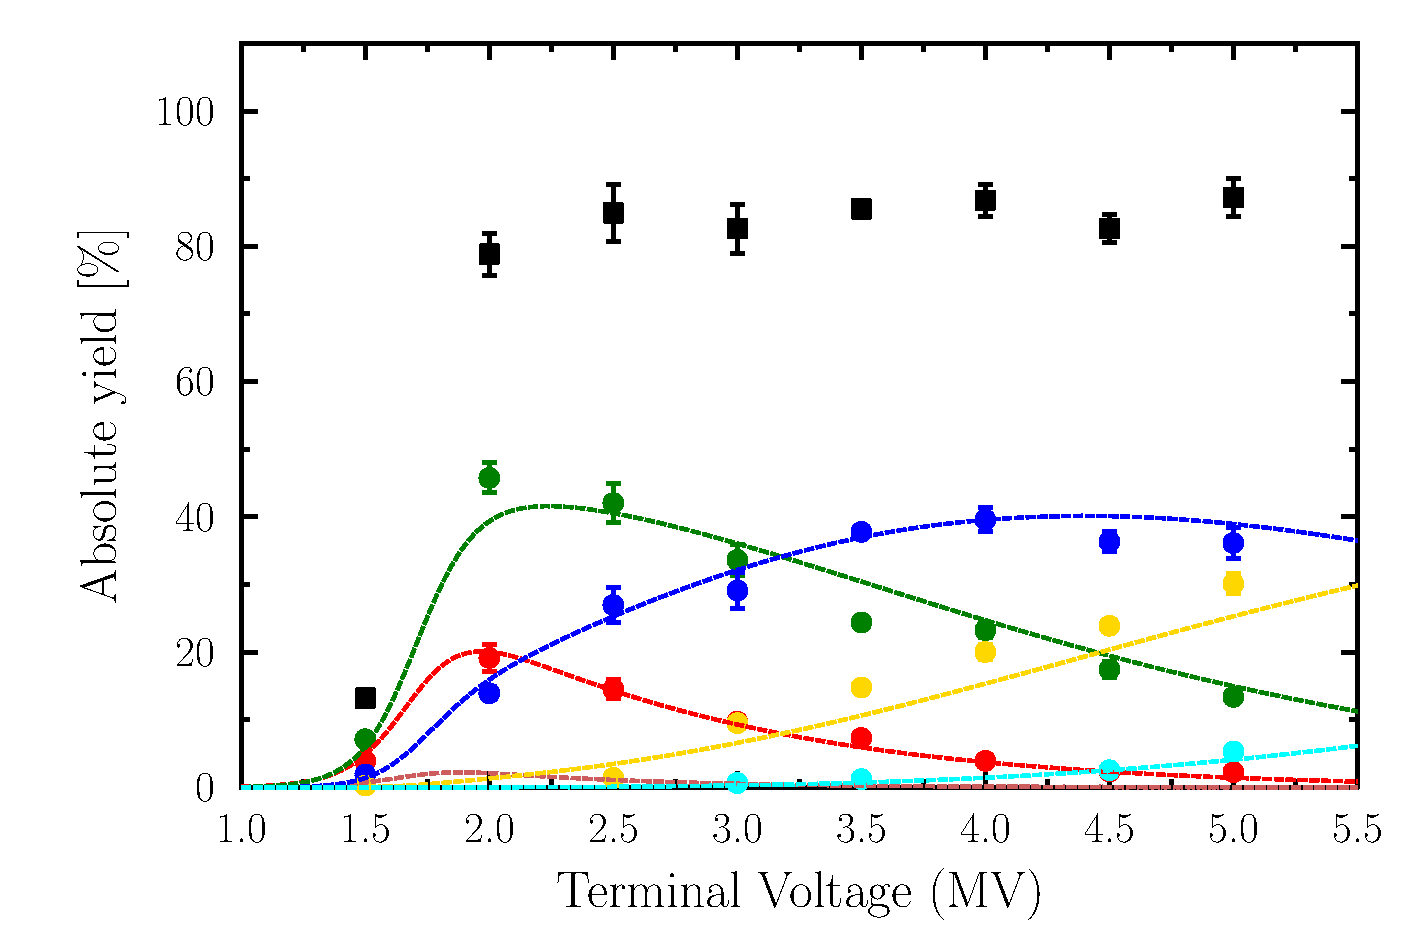
\includegraphics[width=0.75\textwidth]{absolute-16.pdf}      
	\caption{Absolute yield measurements [as a \% of total injected beam]
		for O charge states +1 -- +5 measured from BeO, as a function of terminal
		voltage in MV. Legend -- Measured: $\blacksquare$ -- Total transmission;
		{\protect\tikz[baseline=-0.5ex]\protect\fill[red] (0,0) circle (4pt);} -- +1;
		{\protect\tikz[baseline=-0.5ex]\protect\fill[green] (0,0) circle (4pt);} -- +2;
		{\protect\tikz[baseline=-0.5ex]\protect\fill[blue] (0,0) circle (4pt);} -- +3;
		{\protect\tikz[baseline=-0.5ex]\protect\fill[yellow!60!brown] (0,0) circle (4pt);} -- +4;
		{\protect\tikz[baseline=-0.5ex]\protect\fill[cyan] (0,0) circle (4pt);} -- +5. Error bars shown refer to statistical uncertainty, not machine error.  
		CasP convoluted:
		{\protect\tikz[baseline=-0.5ex]\protect\draw[red!60!brown, very thick, dashed] (0,0) -- (10pt,0);} -- 0;
		{\protect\tikz[baseline=-0.5ex]\protect\draw[red, very thick, dashed] (0,0) -- (10pt,0);} -- +1;
		{\protect\tikz[baseline=-0.5ex]\protect\draw[green, very thick, dashed] (0,0) -- (10pt,0);} -- +2;
		{\protect\tikz[baseline=-0.5ex]\protect\draw[blue, very thick, dashed] (0,0) -- (10pt,0);} -- +3;
		{\protect\tikz[baseline=-0.5ex]\protect\draw[yellow!60!brown, very thick, dashed] (0,0) -- (10pt,0);} -- +4;
		{\protect\tikz[baseline=-0.5ex]\protect\draw[cyan, very thick, dashed] (0,0) -- (10pt,0);} -- +5.}
	\label{fig:abs_yield}
\end{figure}

%%%%%%%%%%%%%%%%%%%%%%%%%%%%%%%%%%%%%%%%%%Relative yield table and figure%%%%%%%%%%%%%%%%%%%%%%%

In Table \ref{table:rel_yield}, the relative yields of oxygen charge states from injected \ce{BeO-} ions are shown. Measurements are made from 1.5 MV to 5 MV in steps of 0.5 MV. In the last two columns, the mean and standard deviation of the resultant Gaussian distribution are presented, for a given terminal voltage. The Gaussian distribution is central to charge state distributions and represents the equilibrium of the many-step charge exchange process. From the measurements of 8 terminal voltages of \ce{BeO-}, we can see the mean charge state increases with increasing ion energy. The width of the Gaussian distributions for \ce{BeO-} show no trend apart from some small changes. In the 9th and 10th rows in Table \ref{table:rel_yield}, we have the relative yields of oxygen charge states from injected \ce{O2-} ions and \ce{O-} ions at 4 MV, and 1.92 MV respectively. They will be discussed in more detail in Figure \ref{fig:molecular_effect} . The last 3 rows in this table are from literature values. 


\begin{table}[h!]
	\begin{threeparttable}		
			\caption{\parbox{0.80\textwidth}{Equilibrium charge fractions $F_q^\text{eq}$ (in \%) of oxygen charge states from injected atomic and molecular negative ions after argon gas stripper. Entries in the last two columns show the parameters of a univariate normal distribution  $\mathcal{N}(\bar{q},\Delta_{\bar{q}})$ fitted to the data. For comparison, the last three rows include previous experimental data \cite{preikschat1966charge,Hubbard1955,Liu2014}.}}
			\label{table:rel_yield}			
			\begin{tabular}{c c c c c c c c c c}
				\toprule
				Injected & Terminal voltage & $E/M$ & \multicolumn{5}{c}{Positive ion charge state $q$} & Mean & std \\
				Ion & $U_T$ (MV) & (MeV/u) & $1+$ & $2+$ & $3+$ & $4+$ & $5+$ & $\bar{q}$ & $\Delta_{\bar{q}}$ \\
				\midrule
				$^{9}$Be$^{16}$O$^-$ & 1.50 & 0.06 & 29.35  & 54.07  & 14.44  & 2.14  &  & 1.89 & 0.72 \\
				& 2.00 & 0.08 & 24.29 & 58.05 & 17.66 &   &  & 1.93 & 0.64 \\
				& 2.50 & 0.10 & 17.10 & 49.48 & 31.75 & 1.67  &  & 2.18 & 0.72 \\
				& 3.00 & 0.12 & 11.76  & 40.72 & 35.23 & 11.51  & 0.79 & 2.49 & 0.87 \\
				& 3.50 & 0.14 & 8.54  & 28.53 & 44.19 & 17.30 & 1.44 & 2.75 & 0.89 \\
				& 4.00 & 0.16 & 4.54  & 26.79 & 45.61 & 23.07 &  & 2.87 & 0.81 \\
				& 4.50 & 0.18 & 2.87  & 21.13 & 43.98 & 28.92 & 3.09 & 3.08 & 0.86 \\
				& 5.00 & 0.20 & 2.59  & 15.36 & 41.43 & 34.52 & 6.09 & 3.26 & 0.88 \\
				\addlinespace				
				$^{16}$O$_2^-$        & 4.00 & 0.13 & 14.83 & 44.76 & 35.91 & 4.49  &  & 2.30 & 0.77 \\
				\addlinespace				
				$^{16}$O$^-$          & 1.92 & 0.12 & 8.65  & 38.35 & 38.70 & 13.75 & 0.55 & 2.59 & 0.85 \\
				\addlinespace				
				\tnote{1} & 2.50 & 0.156 & 0.71  & 35.55 & 47.17 & 16.58 &      & 2.80 & 0.71 \\
				\tnote{2}     & n/a  & 0.203 &       & 12.0  & 38.0  & 39.0  & 11.0 & 3.49 & 0.84 \\
				\tnote{3}     & n/a  & 0.216 & 5.8   & 23.2  & 43.9  & 24.0  & 3.1  & 2.95 & 0.91 \\
				\bottomrule
			\end{tabular}			
			\begin{tablenotes}
				\footnotesize
				\item[1] Injected ion \ce{^{16}O^-} on \ce{O2} stripper gas (charge equilibrium uncertain) \cite{preikschat1966charge}.
				\item[2] Accelerated \ce{^{16}O^{q+}} ions on external Ar gas stripper (charge equilibrium) \cite{Hubbard1955}.
				\item[3] Accelerated \ce{^{16}O^{q+}} ions on external He gas stripper (charge equilibrium) \cite{Liu2014}.
			\end{tablenotes}			
	\end{threeparttable}
\end{table}

In Figure \ref{fig:rel_yield}, we present the relative yields of oxygen charge states as a function of terminal voltage (i.e. energy)  just from injected \ce{BeO-} ions. All measurements were carried out at a stripper gas pressure that was high enough for reaching  equilibrium charge state distribution, so that our relative yields for each charge state $q$ approximate rather well the limiting equilibrium charge fractions $F_q^\text{eq}$ of theoretical models by CasP and Schiwietz and Grande \cite{schiwietz2001improved}. 
A full error analysis has been done for all experimental data points. The error bars can be seen for all our measured points in Figure \ref{fig:rel_yield}.  The uncertainty in the relative yields is then obtained by error propagation calculation and is presented in percentages relative to the values in Figure \ref{fig:rel_yield}. 
The average uncertainty in relative yield for O charge states measured from \ce{BeO-} over all terminal voltages was 1.55 \%. All percentage uncertainties stated here refer to relative uncertainty.

Considering Figure \ref{fig:rel_yield}, starting with the +1 measured data points (red), we can see at 1.5 MV our data point matches that of Schiwietz and Grande. All measurements above 1.5 MV tend to agree more with the predictions of CasP. For +2 measured data points (green), our 2 MV data point is above both predictions, with the rest tending to agree with CasP within error bars. However there are some exceptions such as a 3.5 and 5 MV, our measurement points seem to be closer with that of  Schiwietz and Grande. For +3 (blue) at 1.5 MV we have agreement with Schiwietz and Grande, above that there is agreement within error bars with CasP, but for 4.5 and 5 MV there is more agreement with Schiwietz and Grande. For +4 (yellow) we have agreement with Schiwietz and Grande for all data points except 2.5 MV, which is well below both predictions. Also one should note that from 1.5 - 2.5 MV relative yields are close to 0 and so are not particularly significant. For +5 (light blue) relative yields are quite low until above 4.5 MV, yields are below 5\%. At 5 MV our point agrees with Schiwietz and Grande, however the yield is around 6\%.

In general, we can see that at low energies there is more agreement with Schiwietz and Grande, and at higher energies there's more agreement with the semi-empirical parametrisation in the CasP code. A possible explanation for this can be the low transmission at low terminal voltages.  However one should bear in mind that at low energies we have higher uncertainties and there are extremely low transmissions especially below 2 MV (i.e. refer to Figure \ref{fig:abs_yield}). Reasons for the low transmission are given with regards to the discussion of Figure \ref{fig:abs_yield}. After 2 MV we obtain flat top transmission, which means from 2 MV and above we can be sure that the true and accurate charge state distribution is being measured. Also we see in the cases of +4 and +5 more agreement with  Schiwietz and Grande. There is a different formula used by CasP and by Schiwietz and Grande \cite{PrivComm}, so both of them are calculated slightly differently.      

In addition, comparisons are made against literature values \cite{Hubbard1955,preikschat1966charge,Liu2014}. The experimental setups of these measurements differ from each other and from the current one: Hubbard and Lauer used a separate Ar gas stripper after the accelerator and Preikschat and Cramer \cite{preikschat1966charge} used oxygen gas stripper in a tandem accelerator. Liu et al \cite{Liu2014} used a separate He gas stripper after the main accelerator. Preikschat and Cramer \cite{preikschat1966charge} ‘s data points match ours for +3. For +2 and +4 they don’t. For +1 they are close to 0 and hence meaningless. It's worth noting that all the points in our relative figure have been scaled to 100\%, so if something is overestimated and it drops all other points will go up. 

Hubbard and Lauer measured oxygen charge distributions with an external Ar gas stripper (length 508 mm, diam. 3.175 mm) at an equilibrium target thickness. In terms of their data points +2 is below ours, and +5 is above ours. We can say that the difference is small between their points and ours and considering the fact that the yields are also quite low, it is possible that our points are not too far apart. Also their +4 is above ours and our +3 is above theirs. Although again they are quite close so it might almost be the same result. To our knowledge, this is the only previous experiment at similar conditions to ours reported in the literature. These authors observed that the equilibrium charge distribution is independent of the used stripping gas for oxygen and neon beams at energies of about 7.1 MeV. While this may not be true in general and especially at lower energies, we assume it meaningful to compare our results also with the data from Ref. \cite{preikschat1966charge} although the latter were obtained by using oxygen gas stripper. However, their results may have suffered from beam losses caused by angular straggling because the yields of higher charge states do not saturate to a constant level when the gas pressure is increased. The charge distribution data probably do not correspond to charge equilibrium. The use of a separate, external gas stripper by Hubbard and Lauer seems more beneficial in this respect.

In a recent experiment, Liu et al \cite{Liu2014} studied oxygen charge state distributions in a windowless He gas target of effective length of 44 mm and observed that a target thickness of about 20$\times10^{16}$~atoms/cm$^2$  was required for charge equilibrium at 7.2 MeV oxygen ion energy. Looking at their data we see, it is around 5.5 MV, which is above our measurement range. +3 agrees quite well with CasP. +2 and +4 are bad and don’t even agree with CasP. +1 and +5 are also bad, the ordering and ratios are inverse, and don’t agree with CasP, however the relative yields are quite low. In general we see large deviations between their measurements and the predictions however they use a different stripping gas i.e. He. Their theoretical analysis employs a plane-wave Born approximation to calculate the ionisation cross sections. This is a first order perturbation theory.  To calculate the electron capture cross sections they use a continuum distorted wave approximation. This theory is used to describe heavy-particle collisions. They found out that the electron capture cross sections are reduced as density of the gas target increases. In a dilute gas, excited electron states of the projectile decay before the atom experiences the next collision, while in a dense gas a further collision may result in ionisation. The effect is even more pronounced at lower energies, which might account for larger deviations of experimental measurements from predictions in that energy range.  
 

%Figure
\begin{figure}[h!] 
	\centering
	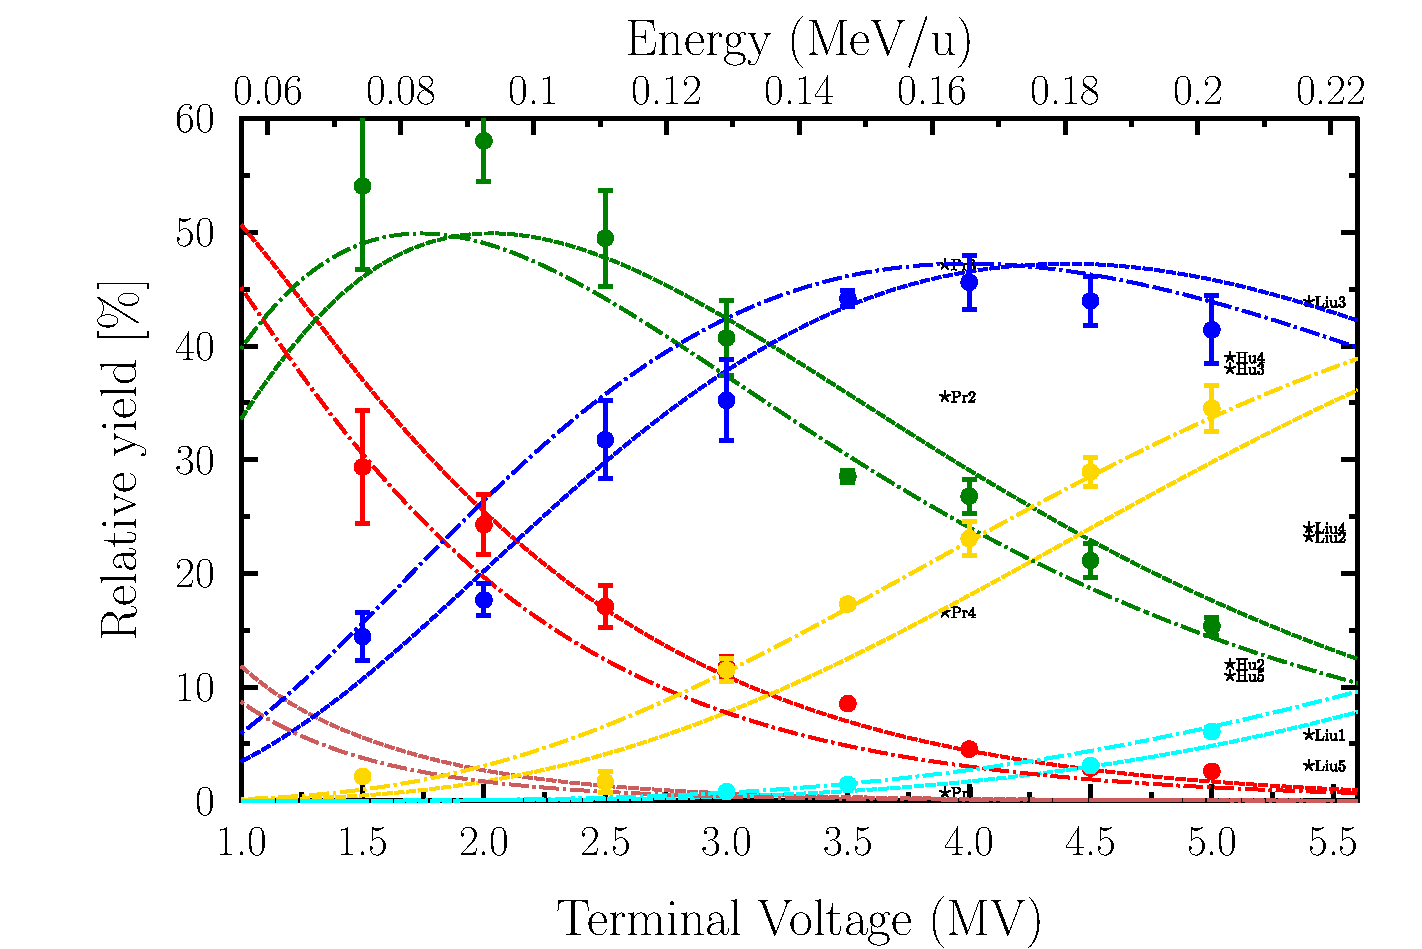
\includegraphics[width=0.75\textwidth]{relative-13}
	\caption{Relative yield measurements [as a \% of total injected beam]
		for O charge states +1 -- +5 measured from BeO. Legend -- Measured: 	{\protect\tikz[baseline=-0.5ex]\protect\fill[red] (0,0) circle (4pt);} -- +1;
		{\protect\tikz[baseline=-0.5ex]\protect\fill[green] (0,0) circle (4pt);} -- +2;
		{\protect\tikz[baseline=-0.5ex]\protect\fill[blue] (0,0) circle (4pt);} -- +3;
		{\protect\tikz[baseline=-0.5ex]\protect\fill[yellow!60!brown] (0,0) circle (4pt);} -- +4;
		{\protect\tikz[baseline=-0.5ex]\protect\fill[cyan] (0,0) circle (4pt);} -- +5. Error bars shown refer to statistical uncertainty.  Experimental data from Preikschat and Cramer \cite{preikschat1966charge} (Pr1-Pr4), Hubbard and Lauer \cite{Hubbard1955} (Hu2-Hu5) and Liu et al. \cite{Liu2014} (Lu1-Lu5)  for atomic \ce{O-} are shown for comparison purposes.  CasP calculations:
		{\protect\tikz[baseline=-0.5ex]\protect\draw[red!60!brown, very thick, dashed] (0,0) -- (10pt,0);} -- 0;
		{\protect\tikz[baseline=-0.5ex]\protect\draw[red, very thick, dashed] (0,0) -- (10pt,0);} -- +1;
		{\protect\tikz[baseline=-0.5ex]\protect\draw[green, very thick, dashed] (0,0) -- (10pt,0);} -- +2;
		{\protect\tikz[baseline=-0.5ex]\protect\draw[blue, very thick, dashed] (0,0) -- (10pt,0);} -- +3;
		{\protect\tikz[baseline=-0.5ex]\protect\draw[yellow!60!brown, very thick, dashed] (0,0) -- (10pt,0);} -- +4;
		{\protect\tikz[baseline=-0.5ex]\protect\draw[cyan, very thick, dashed] (0,0) -- (10pt,0);} -- +5. Schiwietz and Grande \cite{schiwietz2001improved} calculations:{\protect\tikz[baseline=-0.5ex]\protect\draw[red!60!brown, very thick, dotdash] (0,0) -- (10pt,0);} -- 0;
		{\protect\tikz[baseline=-0.5ex]\protect\draw[red, very thick, dotdash] (0,0) -- (10pt,0);} -- +1;
		{\protect\tikz[baseline=-0.5ex]\protect\draw[green, very thick, dotdash] (0,0) -- (10pt,0);} -- +2;
		{\protect\tikz[baseline=-0.5ex]\protect\draw[blue, very thick, dotdash] (0,0) -- (10pt,0);} -- +3;
		{\protect\tikz[baseline=-0.5ex]\protect\draw[yellow!60!brown, very thick, dotdash] (0,0) -- (10pt,0);} -- +4; {\protect\tikz[baseline=-0.5ex]\protect\draw[cyan, very thick, dotdash] (0,0) -- (10pt,0);} -- +5.}\label{fig:rel_yield}
\end{figure}

%%%%%%%%%%%%%%%%%%%%%%%%%%%%%%%%%%%%%%%%%%%Moleular effect figure%%%%%%%%%%%%%%%%%%%%%%%%%

Figure \ref{fig:molecular_effect} shows  relative yields as a function of the oxygen charge states measured from \ce{BeO-} (red square), \ce{O2-} (blue square), and \ce{O-} (green square) at terminal voltages 3 MV, 4 MV, and 1.92 MV, respectively. In Figure \ref{fig:molecular_effect} the shape of the measured charge state distributions follow that of a Gaussian as predicted by Betz \cite{betz1972charge}. Solid lines represent Gaussian fits to experimental data points, using a Scaled Levenberg-Marquardt algorithm. The terminal voltages for \ce{BeO-} and \ce{O2-} were chosen so that in each case the energy of O after molecular break-up at the terminal is comparable to atomic \ce{O-}, i.e., equal to 0.12 MeV/u. Comparisons are made with predictions of the CasP code for oxygen ions impacting Ar gas (black line) at an energy of 120 keV/u which corresponds to the terminal voltage of atomic \ce{O-} at 1.92 MV. The purpose of this figure is to see whether there is any noticeable change in the charge state distribution of oxygen ions depending on the precursor i.e.the originating species being \ce{BeO-}, \ce{O2-} and  \ce{O-} . This is known as the "molecular effect”. 


%Figure
\begin{figure}[h!] 
	\centering
		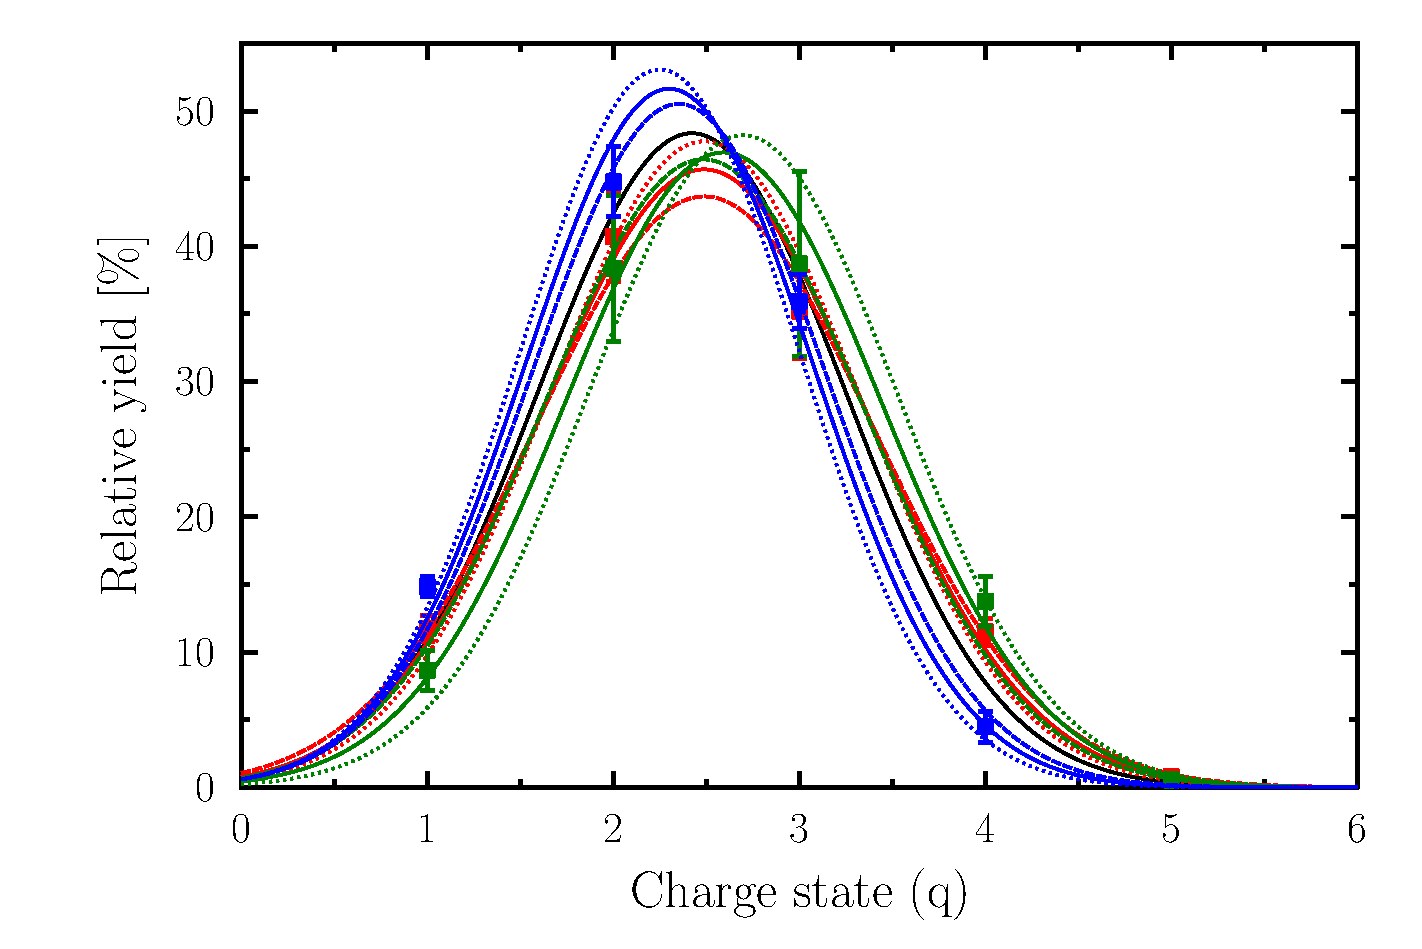
\includegraphics[width=0.75\textwidth]{s4_mol-effect-04}
\caption{
	Comparison of oxygen charge state distributions, from oxygen of three different species 
	(\ce{BeO-}, \ce{O2-}, and \ce{O-}), all at the same energy. 
	Legend -- Measured: 
	{\protect\tikz[baseline=-0.5ex]\protect\fill[red] (-4pt,-4pt) rectangle (4pt,4pt);} 
	-- \ce{BeO-}, 3 MV; {\protect\tikz[baseline=-0.5ex]\protect\fill[green] (-4pt,-4pt) rectangle (4pt,4pt);} 
	-- \ce{O-}, 1.92 MV;
	{\protect\tikz[baseline=-0.5ex]\protect\fill[blue] (-4pt,-4pt) rectangle (4pt,4pt);} 
	-- \ce{O2-}, 4 MV; Error bars shown refer to statistical uncertainty. Calculated:  {\protect\tikz[baseline=-0.5ex]\protect\draw[black] (0,0) -- (10pt,0);} -- CasP 3 MV $Z_p=8$, $Z_t=18$. Fit: 
	{\protect\tikz[baseline=-0.5ex]\protect\draw[red] (0,0) -- (10pt,0);} -- \ce{BeO-}
	{\protect\tikz[baseline=-0.5ex]\protect\draw[green] (0,0) -- (10pt,0);} -- \ce{O-}
	{\protect\tikz[baseline=-0.5ex]\protect\draw[blue] (0,0) -- (10pt,0);} -- \ce{O2-}. Upper fit:
	{\protect\tikz[baseline=-0.5ex]\protect\draw[red, very thick, dotted] (0,0) -- (10pt,0);} -- \ce{BeO-};
	{\protect\tikz[baseline=-0.5ex]\protect\draw[green, very thick, dotted] (0,0) -- (10pt,0);} -- \ce{O-};
	{\protect\tikz[baseline=-0.5ex]\protect\draw[blue, very thick, dotted] (0,0) -- (10pt,0);} -- \ce{O2-}; Lower fit:
	{\protect\tikz[baseline=-0.5ex]\protect\draw[red, very thick, dashed] (0,0) -- (10pt,0);} -- \ce{BeO-};
	{\protect\tikz[baseline=-0.5ex]\protect\draw[green, very thick, dashed] (0,0) -- (10pt,0);} -- \ce{O-};
	{\protect\tikz[baseline=-0.5ex]\protect\draw[blue, very thick, dashed] (0,0) -- (10pt,0);} -- \ce{O2-}.	
	}
\label{fig:molecular_effect}
	
\end{figure}

An important aspect in  being able to detect any molecular effect is to quantify the uncertainties of the measured points. We have calculated the statistical uncertainty on all measured points in Figure \ref{fig:molecular_effect}  these can be seen in the form of error bars.  In order to get the maximum extent of the uncertainty we have fitted two additional curves  to our Gaussian fit of the experimental data points.  Therefore for each Gaussian fit of the experimental data point set at a particular terminal voltage, we have an upper fit and a lower fit. The upper fit consists of fitting the points of the first two upper limits of the error bars with the second two lower limits of the error bars. The lower fit consists of the opposite which means fitting the first two lower limits of the error bars with the second two upper limits of the error bars. For each charge state distribution we really only have four data points to work with (+5 is close to zero). By carrying out this procedure we are able to overestimate our uncertainty on the means and standard deviations of our experimental data sets. By taking the differences of the upper and lower fits we are able to determine the errors on the means and standard deviations of our experimental data Gaussian fits. This is known as the "maximum-minimum" method of error analysis. Although this method overestimates the error, it strengthens the validity of our result. A similar process is used to find the errors on the widths of the measured charge state distributions.   

The results of the mean show for CasP we have 2.422; for \ce{BeO-} we have 2.4884 $\pm$ 0.0007; for \ce{O-} we have 2.5920 $\pm$ 0.2127 and for \ce{O2-} we have  2.3006 $\pm$ 0.1020. Here we can see that  \ce{BeO-} has the lowest uncertainty followed by \ce{O2-} and lastly \ce{O-} which has the greatest uncertainty. The means are closest between CasP and \ce{BeO-},  which is surprising because CasP calculates charge state distributions for atomic species  not molecular species, CasP should be closest to \ce{O-}. It is still possible that is still the case because the error bars for \ce{O-} are quite large, so that the means can fall within error range.  We would also like to point out that +2 of \ce{O2-} in Figure \ref{fig:molecular_effect} is far more pronounced and is the highest of all measured yields. If we compare the means of  \ce{BeO-}  and  \ce{O-} they are within the uncertainties so can be considered to be the same. If we compare the means of  \ce{O2-}   and  \ce{O-} they are within the uncertainties so can be considered to be the same. As molecular effect is understood to mean a difference between an atomic and molecular species, in our case within uncertainties there is no difference, so we do not observe a molecular effect within our uncertainty range. When comparing the width of these three distributions (c.f. Table \ref{table:rel_yield}), we can see that the width of the \ce{O2-} distribution is 0.7725 $\pm$ 0.1020 which is narrower, whereas the width for \ce{BeO-} 0.8732 $\pm$  0.09178 and with for \ce{O-}  0.8499 $\pm$ 0.212 are quite similar. However when taking into account uncertainties, we can say they are all within error bounds. The width of CasP is 0.825, which is closer to \ce{O-} and \ce{BeO-}.  




%%%%%%%%%%%%%%%%%%%%%%%%%%%%%%%%%%%%%%%%%%%%%%%%%%%%%%%%%%%%%%%%%%%%%%%%%%%%%

\section{Conclusion}


In this study, oxygen charge state distributions from a tandem accelerator using Ar stripper gas at terminal voltages of $2-5$ MV were measured. Negative ions when oxygen was injected in the accelerator of both atomic (\ce{O-}) and molecular (\ce{BeO-}, and \ce{O2-}) form were used. Absolute yields were measured  along with total transmissions. For the measured range, transmission holds at around 80\% except for between 2 - 1.5 MV where we observe a step-drop to about 15\%.  It was found out for oxygen ions transmission drops steeply between 1.5 and 2 MV. +2 is the most abundant oxygen charge state up to 3.2 MV after which +3 becomes the most abundant charge state. This can be valid for all types of ions that may be measured by AMS. Though molecular ions may still affect non-equilibrium charge distributions, especially in solid strippers. 


We obtained a series of symmetric Gaussian distributions as it is expected from charge state distribution theory. Relative yields of charge states $q=+1$ to $+5$ were determined and compared to semi-empirical predictions of CasP code and the Schiwietz and Grande formula. In general, the measured values follow the same trend as the predicted values. Although we obtained a good general agreement within uncertainty, there were certain regions where agreement was better with Schiwietz and Grande and others where agreement was better with CasP . However, we still believe that CasP is a good tool for predicting and planning future experiments. The main factors affecting the charge state yield are the velocity of the ion and the interactions between the electrons of the ion and the electrons of the stripper medium.




% To print the credit authorship contribution details
\printcredits

%% Loading bibliography style file
%\bibliographystyle{model1-num-names}{cas-model2-names}
\bibliographystyle{unsrt}

%\section*{References}
% Loading bibliography database
\bibliography{mybibfile}

%% Biography
%\bio{}
%% Here goes the biography details.
%\endbio
%
%%\bio{pic1}
%% Here goes the biography details.
%\endbio

\end{document}



